\documentclass{standalone}
\usepackage{tikz}
\usetikzlibrary{patterns, positioning}


\begin{document}
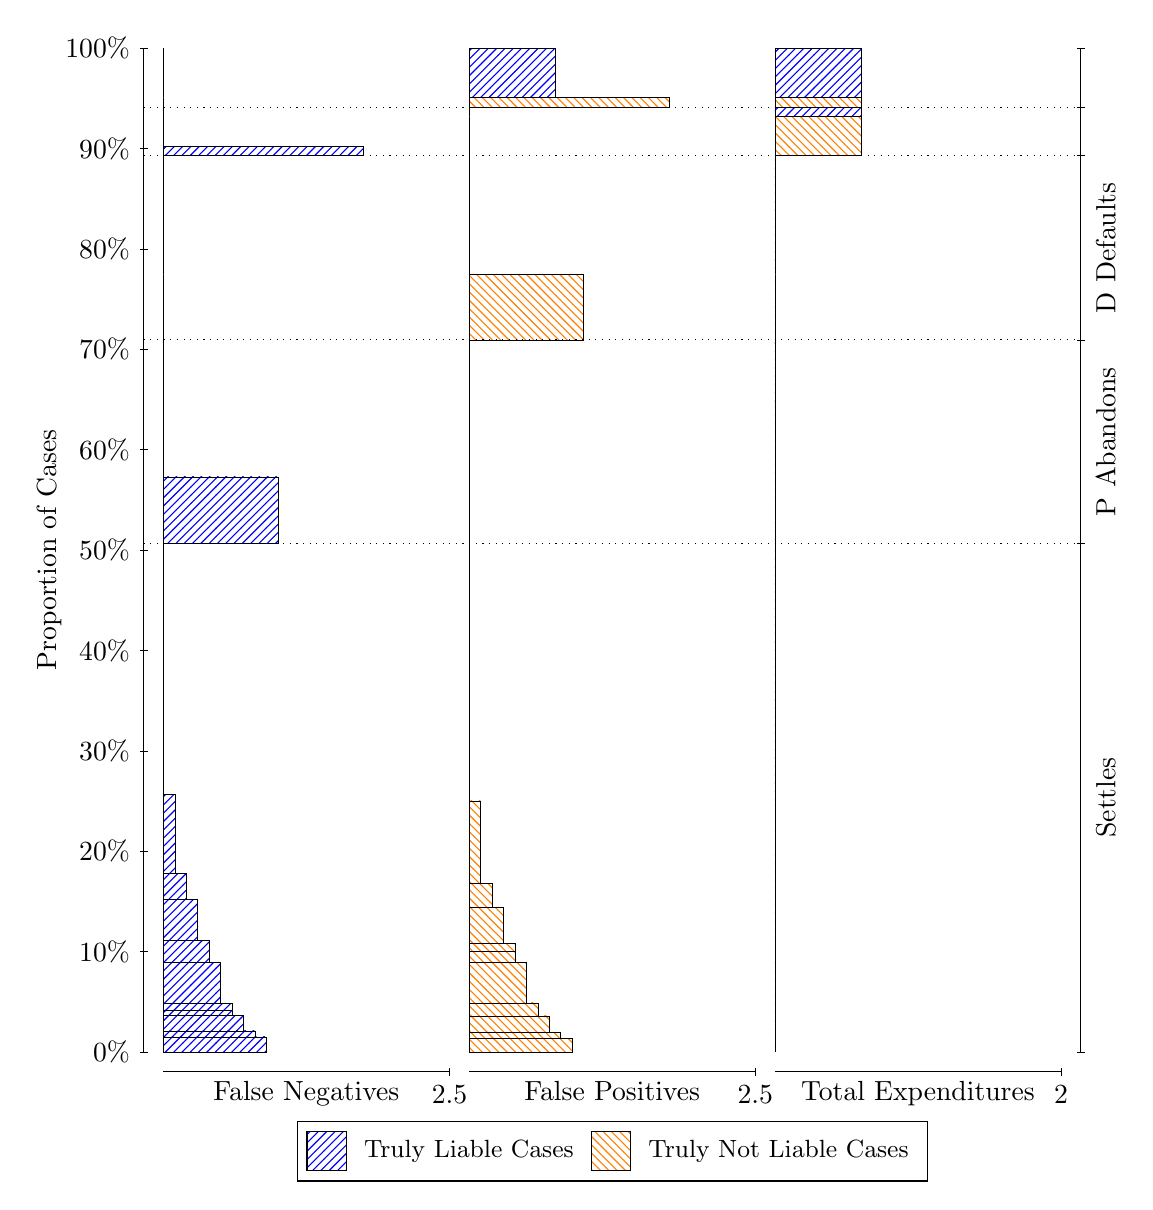
\begin{tikzpicture}
\draw[black, very thin] (1.5,1.75) -- (1.5,14.5);
\node[rotate=90, text=black, anchor=center] at (0.3, 8.125) {Proportion of Cases};
\draw[black, very thin] (1.45,1.75) -- (1.55,1.75);
\node[text=black, anchor=east] at (1.45, 1.75) {0\%};
\draw[black, very thin] (1.45,3.025) -- (1.55,3.025);
\node[text=black, anchor=east] at (1.45, 3.025) {10\%};
\draw[black, very thin] (1.45,4.3) -- (1.55,4.3);
\node[text=black, anchor=east] at (1.45, 4.3) {20\%};
\draw[black, very thin] (1.45,5.575) -- (1.55,5.575);
\node[text=black, anchor=east] at (1.45, 5.575) {30\%};
\draw[black, very thin] (1.45,6.85) -- (1.55,6.85);
\node[text=black, anchor=east] at (1.45, 6.85) {40\%};
\draw[black, very thin] (1.45,8.125) -- (1.55,8.125);
\node[text=black, anchor=east] at (1.45, 8.125) {50\%};
\draw[black, very thin] (1.45,9.4) -- (1.55,9.4);
\node[text=black, anchor=east] at (1.45, 9.4) {60\%};
\draw[black, very thin] (1.45,10.675) -- (1.55,10.675);
\node[text=black, anchor=east] at (1.45, 10.675) {70\%};
\draw[black, very thin] (1.45,11.95) -- (1.55,11.95);
\node[text=black, anchor=east] at (1.45, 11.95) {80\%};
\draw[black, very thin] (1.45,13.225) -- (1.55,13.225);
\node[text=black, anchor=east] at (1.45, 13.225) {90\%};
\draw[black, very thin] (1.45,14.5) -- (1.55,14.5);
\node[text=black, anchor=east] at (1.45, 14.5) {100\%};

\draw[black, very thin] (13.4,1.75) -- (13.4,14.5);
\draw[black, very thin] (13.35,1.75) -- (13.45,1.75);
\node[anchor=west] at (13.35, 1.75) {};
\draw[black, very thin] (13.35,8.2108) -- (13.45,8.2108);
\node[anchor=west] at (13.35, 8.2108) {};
\draw[black, very thin] (13.35,10.793) -- (13.45,10.793);
\node[anchor=west] at (13.35, 10.793) {};
\draw[black, very thin] (13.35,13.133) -- (13.45,13.133);
\node[anchor=west] at (13.35, 13.133) {};
\draw[black, very thin] (13.35,13.749) -- (13.45,13.749);
\node[anchor=west] at (13.35, 13.749) {};
\draw[black, very thin] (13.35,14.5) -- (13.45,14.5);
\node[anchor=west] at (13.35, 14.5) {};

\draw[black, very thin, pattern color=blue, pattern=north east lines] (1.75,1.75) rectangle (3.058,1.9409);
\draw[black, very thin, pattern color=blue, pattern=north east lines] (1.75,1.9409) rectangle (2.9127,2.0174);
\draw[black, very thin, pattern color=blue, pattern=north east lines] (1.75,2.0174) rectangle (2.7673,2.2099);
\draw[black, very thin, pattern color=blue, pattern=north east lines] (1.75,2.2099) rectangle (2.622,2.277);
\draw[black, very thin, pattern color=blue, pattern=north east lines] (1.75,2.277) rectangle (2.622,2.3687);
\draw[black, very thin, pattern color=blue, pattern=north east lines] (1.75,2.3687) rectangle (2.4767,2.886);
\draw[black, very thin, pattern color=blue, pattern=north east lines] (1.75,2.886) rectangle (2.3313,3.1651);
\draw[black, very thin, pattern color=blue, pattern=north east lines] (1.75,3.1651) rectangle (2.186,3.69);
\draw[black, very thin, pattern color=blue, pattern=north east lines] (1.75,3.69) rectangle (2.0407,4.0187);
\draw[black, very thin, pattern color=blue, pattern=north east lines] (1.75,4.0187) rectangle (1.8953,5.0224);
\draw[black, very thin, pattern color=orange, pattern=north west lines] (1.75,5.0224) rectangle (1.75,8.2108);
\draw[black, very thin, pattern color=blue, pattern=north east lines] (1.75,8.2108) rectangle (3.2033,9.0532);
\draw[black, very thin, pattern color=orange, pattern=north west lines] (1.75,9.0532) rectangle (1.75,10.793);
\draw[black, very thin, pattern color=orange, pattern=north west lines] (1.75,10.793) rectangle (1.75,11.623);
\draw[black, very thin, pattern color=blue, pattern=north east lines] (1.75,11.623) rectangle (1.75,13.133);
\draw[black, very thin, pattern color=blue, pattern=north east lines] (1.75,13.133) rectangle (4.2933,13.254);
\draw[black, very thin, pattern color=orange, pattern=north west lines] (1.75,13.254) rectangle (1.75,13.749);
\draw[black, very thin, pattern color=orange, pattern=north west lines] (1.75,13.749) rectangle (1.75,13.871);
\draw[black, very thin, pattern color=blue, pattern=north east lines] (1.75,13.871) rectangle (1.75,14.5);
\draw[black, very thin, pattern color=orange, pattern=north west lines] (5.6333,1.75) rectangle (6.9413,1.9229);
\draw[black, very thin, pattern color=orange, pattern=north west lines] (5.6333,1.9229) rectangle (6.796,2.0006);
\draw[black, very thin, pattern color=orange, pattern=north west lines] (5.6333,2.0006) rectangle (6.6507,2.2094);
\draw[black, very thin, pattern color=orange, pattern=north west lines] (5.6333,2.2094) rectangle (6.5053,2.3734);
\draw[black, very thin, pattern color=orange, pattern=north west lines] (5.6333,2.3734) rectangle (6.36,2.8863);
\draw[black, very thin, pattern color=orange, pattern=north west lines] (5.6333,2.8863) rectangle (6.2147,3.0275);
\draw[black, very thin, pattern color=orange, pattern=north west lines] (5.6333,3.0275) rectangle (6.2147,3.1255);
\draw[black, very thin, pattern color=orange, pattern=north west lines] (5.6333,3.1255) rectangle (6.0693,3.5839);
\draw[black, very thin, pattern color=orange, pattern=north west lines] (5.6333,3.5839) rectangle (5.924,3.8869);
\draw[black, very thin, pattern color=orange, pattern=north west lines] (5.6333,3.8869) rectangle (5.7787,4.9383);
\draw[black, very thin, pattern color=blue, pattern=north east lines] (5.6333,4.9383) rectangle (5.6333,8.2108);
\draw[black, very thin, pattern color=orange, pattern=north west lines] (5.6333,8.2108) rectangle (5.6333,9.9507);
\draw[black, very thin, pattern color=blue, pattern=north east lines] (5.6333,9.9507) rectangle (5.6333,10.793);
\draw[black, very thin, pattern color=orange, pattern=north west lines] (5.6333,10.793) rectangle (7.0867,11.623);
\draw[black, very thin, pattern color=blue, pattern=north east lines] (5.6333,11.623) rectangle (5.6333,13.133);
\draw[black, very thin, pattern color=orange, pattern=north west lines] (5.6333,13.133) rectangle (5.6333,13.628);
\draw[black, very thin, pattern color=blue, pattern=north east lines] (5.6333,13.628) rectangle (5.6333,13.749);
\draw[black, very thin, pattern color=orange, pattern=north west lines] (5.6333,13.749) rectangle (8.1767,13.871);
\draw[black, very thin, pattern color=blue, pattern=north east lines] (5.6333,13.871) rectangle (6.7233,14.5);
\draw[black, very thin, pattern color=orange, pattern=north west lines] (9.5167,1.75) rectangle (9.5167,4.9383);
\draw[black, very thin, pattern color=blue, pattern=north east lines] (9.5167,4.9383) rectangle (9.5167,8.2108);
\draw[black, very thin, pattern color=orange, pattern=north west lines] (9.5167,8.2108) rectangle (9.5167,9.9507);
\draw[black, very thin, pattern color=blue, pattern=north east lines] (9.5167,9.9507) rectangle (9.5167,10.793);
\draw[black, very thin, pattern color=orange, pattern=north west lines] (9.5167,10.793) rectangle (9.5167,11.623);
\draw[black, very thin, pattern color=blue, pattern=north east lines] (9.5167,11.623) rectangle (9.5167,13.133);
\draw[black, very thin, pattern color=orange, pattern=north west lines] (9.5167,13.133) rectangle (10.607,13.628);
\draw[black, very thin, pattern color=blue, pattern=north east lines] (9.5167,13.628) rectangle (10.607,13.749);
\draw[black, very thin, pattern color=orange, pattern=north west lines] (9.5167,13.749) rectangle (10.607,13.871);
\draw[black, very thin, pattern color=blue, pattern=north east lines] (9.5167,13.871) rectangle (10.607,14.5);
\draw[black, dotted] (1.5,8.2108) -- (13.4,8.2108);
\draw[black, dotted] (1.5,10.793) -- (13.4,10.793);
\draw[black, dotted] (1.5,13.133) -- (13.4,13.133);
\draw[black, dotted] (1.5,13.749) -- (13.4,13.749);
\draw[black, very thin] (1.75,1.5) -- (5.3833,1.5);
\node[text=black, anchor=north] at (3.5667, 1.5) {False Negatives};
\draw[black, very thin] (5.3833,1.45) -- (5.3833,1.55);
\node[text=black, anchor=north] at (5.3833, 1.45) {2.5};

\draw[black, very thin] (5.6333,1.5) -- (9.2667,1.5);
\node[text=black, anchor=north] at (7.45, 1.5) {False Positives};
\draw[black, very thin] (9.2667,1.45) -- (9.2667,1.55);
\node[text=black, anchor=north] at (9.2667, 1.45) {2.5};

\draw[black, very thin] (9.5167,1.5) -- (13.15,1.5);
\node[text=black, anchor=north] at (11.333, 1.5) {Total Expenditures};
\draw[black, very thin] (13.15,1.45) -- (13.15,1.55);
\node[text=black, anchor=north] at (13.15, 1.45) {2};

\node[text=black, centered, rotate=90] at (13.72, 4.9804) {Settles};
\node[text=black, centered, rotate=90] at (13.72, 9.5019) {P Abandons};
\node[text=black, centered, rotate=90] at (13.72, 11.963) {D Defaults};



\draw (7.449999999999999,1.5) node[draw=none] (baseCoordinate) {};
\begin{scope}[align=center]
        \matrix[scale=0.5, draw=black, below=0.5cm of baseCoordinate, nodes={draw}, column sep=0.1cm]{
            \node[rectangle, draw, minimum width=0.5cm, minimum height=0.5cm, pattern color=blue, pattern=north east lines] {}; &
            \node[draw=none, font=\small, text=black] (B) {Truly Liable Cases}; &
            \node[rectangle, draw, minimum width=0.5cm, minimum height=0.5cm, pattern color=orange, pattern=north west lines] {}; &
            \node[draw=none, font=\small, text=black] (B) {Truly Not Liable Cases}; \\
            };
\end{scope}

\end{tikzpicture}
\end{document}